\documentclass[class=minimal,border=0pt]{standalone}
\usepackage{hyperref}
\hypersetup{
colorlinks=true,
urlcolor=cyan}
\usepackage{tikz}
\begin{document}
%\documentclass{standalone}
%\usepackage{tikz}
%\usetikzlibrary{patterns,plotmarks}
%\begin{document}
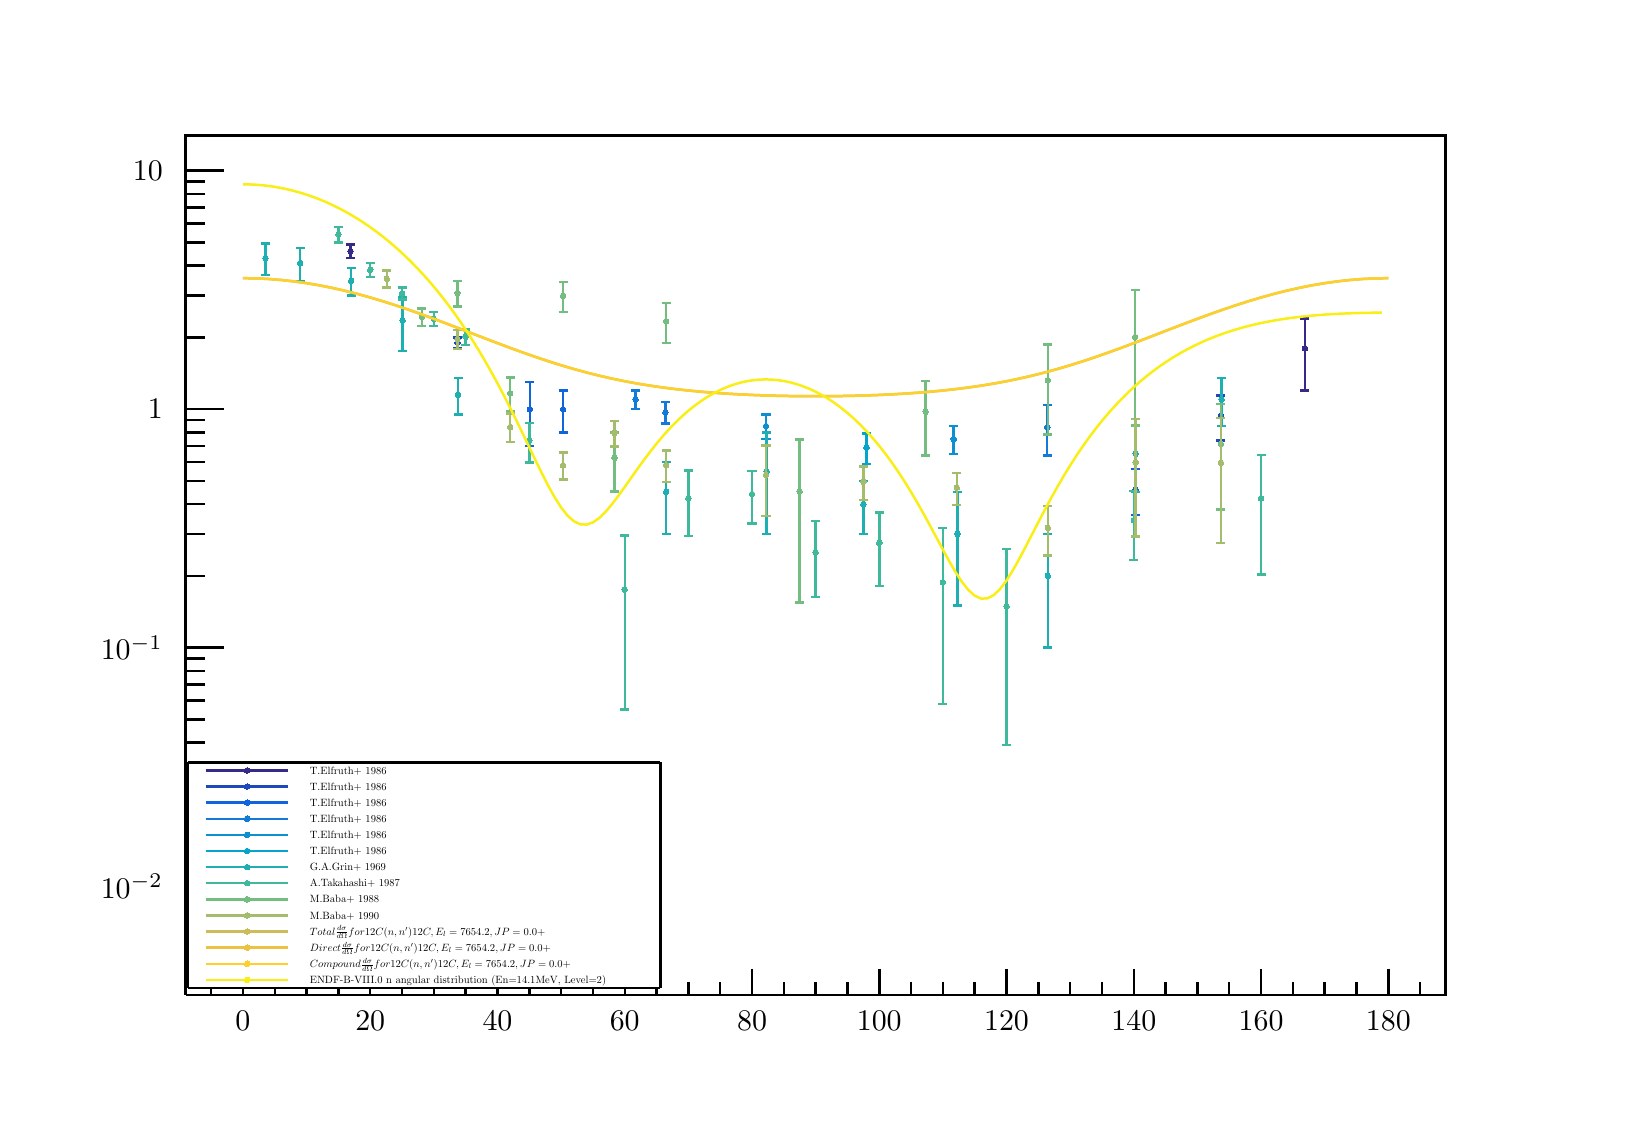
\begin{tikzpicture}
\def\CheckTikzLibraryLoaded#1{ \ifcsname tikz@library@#1@loaded\endcsname \else \PackageWarning{tikz}{usetikzlibrary{#1} is missing in the preamble.} \fi }
\CheckTikzLibraryLoaded{patterns}
\CheckTikzLibraryLoaded{plotmarks}
\pgfdeclareplotmark{cross} {
\pgfpathmoveto{\pgfpoint{-0.3\pgfplotmarksize}{\pgfplotmarksize}}
\pgfpathlineto{\pgfpoint{+0.3\pgfplotmarksize}{\pgfplotmarksize}}
\pgfpathlineto{\pgfpoint{+0.3\pgfplotmarksize}{0.3\pgfplotmarksize}}
\pgfpathlineto{\pgfpoint{+1\pgfplotmarksize}{0.3\pgfplotmarksize}}
\pgfpathlineto{\pgfpoint{+1\pgfplotmarksize}{-0.3\pgfplotmarksize}}
\pgfpathlineto{\pgfpoint{+0.3\pgfplotmarksize}{-0.3\pgfplotmarksize}}
\pgfpathlineto{\pgfpoint{+0.3\pgfplotmarksize}{-1.\pgfplotmarksize}}
\pgfpathlineto{\pgfpoint{-0.3\pgfplotmarksize}{-1.\pgfplotmarksize}}
\pgfpathlineto{\pgfpoint{-0.3\pgfplotmarksize}{-0.3\pgfplotmarksize}}
\pgfpathlineto{\pgfpoint{-1.\pgfplotmarksize}{-0.3\pgfplotmarksize}}
\pgfpathlineto{\pgfpoint{-1.\pgfplotmarksize}{0.3\pgfplotmarksize}}
\pgfpathlineto{\pgfpoint{-0.3\pgfplotmarksize}{0.3\pgfplotmarksize}}
\pgfpathclose
\pgfusepathqstroke
}
\pgfdeclareplotmark{cross*} {
\pgfpathmoveto{\pgfpoint{-0.3\pgfplotmarksize}{\pgfplotmarksize}}
\pgfpathlineto{\pgfpoint{+0.3\pgfplotmarksize}{\pgfplotmarksize}}
\pgfpathlineto{\pgfpoint{+0.3\pgfplotmarksize}{0.3\pgfplotmarksize}}
\pgfpathlineto{\pgfpoint{+1\pgfplotmarksize}{0.3\pgfplotmarksize}}
\pgfpathlineto{\pgfpoint{+1\pgfplotmarksize}{-0.3\pgfplotmarksize}}
\pgfpathlineto{\pgfpoint{+0.3\pgfplotmarksize}{-0.3\pgfplotmarksize}}
\pgfpathlineto{\pgfpoint{+0.3\pgfplotmarksize}{-1.\pgfplotmarksize}}
\pgfpathlineto{\pgfpoint{-0.3\pgfplotmarksize}{-1.\pgfplotmarksize}}
\pgfpathlineto{\pgfpoint{-0.3\pgfplotmarksize}{-0.3\pgfplotmarksize}}
\pgfpathlineto{\pgfpoint{-1.\pgfplotmarksize}{-0.3\pgfplotmarksize}}
\pgfpathlineto{\pgfpoint{-1.\pgfplotmarksize}{0.3\pgfplotmarksize}}
\pgfpathlineto{\pgfpoint{-0.3\pgfplotmarksize}{0.3\pgfplotmarksize}}
\pgfpathclose
\pgfusepathqfillstroke
}
\pgfdeclareplotmark{newstar} {
\pgfpathmoveto{\pgfqpoint{0pt}{\pgfplotmarksize}}
\pgfpathlineto{\pgfqpointpolar{44}{0.5\pgfplotmarksize}}
\pgfpathlineto{\pgfqpointpolar{18}{\pgfplotmarksize}}
\pgfpathlineto{\pgfqpointpolar{-20}{0.5\pgfplotmarksize}}
\pgfpathlineto{\pgfqpointpolar{-54}{\pgfplotmarksize}}
\pgfpathlineto{\pgfqpointpolar{-90}{0.5\pgfplotmarksize}}
\pgfpathlineto{\pgfqpointpolar{234}{\pgfplotmarksize}}
\pgfpathlineto{\pgfqpointpolar{198}{0.5\pgfplotmarksize}}
\pgfpathlineto{\pgfqpointpolar{162}{\pgfplotmarksize}}
\pgfpathlineto{\pgfqpointpolar{134}{0.5\pgfplotmarksize}}
\pgfpathclose
\pgfusepathqstroke
}
\pgfdeclareplotmark{newstar*} {
\pgfpathmoveto{\pgfqpoint{0pt}{\pgfplotmarksize}}
\pgfpathlineto{\pgfqpointpolar{44}{0.5\pgfplotmarksize}}
\pgfpathlineto{\pgfqpointpolar{18}{\pgfplotmarksize}}
\pgfpathlineto{\pgfqpointpolar{-20}{0.5\pgfplotmarksize}}
\pgfpathlineto{\pgfqpointpolar{-54}{\pgfplotmarksize}}
\pgfpathlineto{\pgfqpointpolar{-90}{0.5\pgfplotmarksize}}
\pgfpathlineto{\pgfqpointpolar{234}{\pgfplotmarksize}}
\pgfpathlineto{\pgfqpointpolar{198}{0.5\pgfplotmarksize}}
\pgfpathlineto{\pgfqpointpolar{162}{\pgfplotmarksize}}
\pgfpathlineto{\pgfqpointpolar{134}{0.5\pgfplotmarksize}}
\pgfpathclose
\pgfusepathqfillstroke
}
\definecolor{c}{rgb}{1,1,1};
\draw [color=c, fill=c] (0,0) rectangle (20,13.639);
\draw [color=c, fill=c] (2,1.3639) rectangle (18,12.2751);
\definecolor{c}{rgb}{0,0,0};
\draw [c,line width=0.9] (2,1.3639) -- (2,12.2751) -- (18,12.2751) -- (18,1.3639) -- (2,1.3639);
\draw [c,line width=0.9] (2,1.3639) -- (18,1.3639);
\draw [c,line width=0.9] (2.72727,1.69123) -- (2.72727,1.3639);
\draw [c,line width=0.9] (3.13131,1.52756) -- (3.13131,1.3639);
\draw [c,line width=0.9] (3.53535,1.52756) -- (3.53535,1.3639);
\draw [c,line width=0.9] (3.93939,1.52756) -- (3.93939,1.3639);
\draw [c,line width=0.9] (4.34343,1.69123) -- (4.34343,1.3639);
\draw [c,line width=0.9] (4.74747,1.52756) -- (4.74747,1.3639);
\draw [c,line width=0.9] (5.15152,1.52756) -- (5.15152,1.3639);
\draw [c,line width=0.9] (5.55556,1.52756) -- (5.55556,1.3639);
\draw [c,line width=0.9] (5.9596,1.69123) -- (5.9596,1.3639);
\draw [c,line width=0.9] (6.36364,1.52756) -- (6.36364,1.3639);
\draw [c,line width=0.9] (6.76768,1.52756) -- (6.76768,1.3639);
\draw [c,line width=0.9] (7.17172,1.52756) -- (7.17172,1.3639);
\draw [c,line width=0.9] (7.57576,1.69123) -- (7.57576,1.3639);
\draw [c,line width=0.9] (7.9798,1.52756) -- (7.9798,1.3639);
\draw [c,line width=0.9] (8.38384,1.52756) -- (8.38384,1.3639);
\draw [c,line width=0.9] (8.78788,1.52756) -- (8.78788,1.3639);
\draw [c,line width=0.9] (9.19192,1.69123) -- (9.19192,1.3639);
\draw [c,line width=0.9] (9.59596,1.52756) -- (9.59596,1.3639);
\draw [c,line width=0.9] (10,1.52756) -- (10,1.3639);
\draw [c,line width=0.9] (10.404,1.52756) -- (10.404,1.3639);
\draw [c,line width=0.9] (10.8081,1.69123) -- (10.8081,1.3639);
\draw [c,line width=0.9] (11.2121,1.52756) -- (11.2121,1.3639);
\draw [c,line width=0.9] (11.6162,1.52756) -- (11.6162,1.3639);
\draw [c,line width=0.9] (12.0202,1.52756) -- (12.0202,1.3639);
\draw [c,line width=0.9] (12.4242,1.69123) -- (12.4242,1.3639);
\draw [c,line width=0.9] (12.8283,1.52756) -- (12.8283,1.3639);
\draw [c,line width=0.9] (13.2323,1.52756) -- (13.2323,1.3639);
\draw [c,line width=0.9] (13.6364,1.52756) -- (13.6364,1.3639);
\draw [c,line width=0.9] (14.0404,1.69123) -- (14.0404,1.3639);
\draw [c,line width=0.9] (14.4444,1.52756) -- (14.4444,1.3639);
\draw [c,line width=0.9] (14.8485,1.52756) -- (14.8485,1.3639);
\draw [c,line width=0.9] (15.2525,1.52756) -- (15.2525,1.3639);
\draw [c,line width=0.9] (15.6566,1.69123) -- (15.6566,1.3639);
\draw [c,line width=0.9] (16.0606,1.52756) -- (16.0606,1.3639);
\draw [c,line width=0.9] (16.4646,1.52756) -- (16.4646,1.3639);
\draw [c,line width=0.9] (16.8687,1.52756) -- (16.8687,1.3639);
\draw [c,line width=0.9] (17.2727,1.69123) -- (17.2727,1.3639);
\draw [c,line width=0.9] (2.72727,1.69123) -- (2.72727,1.3639);
\draw [c,line width=0.9] (2.32323,1.52756) -- (2.32323,1.3639);
\draw [c,line width=0.9] (17.2727,1.69123) -- (17.2727,1.3639);
\draw [c,line width=0.9] (17.6768,1.52756) -- (17.6768,1.3639);
\draw [anchor=base] (2.72727,0.913811) node[scale=1.08185, color=c, rotate=0]{0};
\draw [anchor=base] (4.34343,0.913811) node[scale=1.08185, color=c, rotate=0]{20};
\draw [anchor=base] (5.9596,0.913811) node[scale=1.08185, color=c, rotate=0]{40};
\draw [anchor=base] (7.57576,0.913811) node[scale=1.08185, color=c, rotate=0]{60};
\draw [anchor=base] (9.19192,0.913811) node[scale=1.08185, color=c, rotate=0]{80};
\draw [anchor=base] (10.8081,0.913811) node[scale=1.08185, color=c, rotate=0]{100};
\draw [anchor=base] (12.4242,0.913811) node[scale=1.08185, color=c, rotate=0]{120};
\draw [anchor=base] (14.0404,0.913811) node[scale=1.08185, color=c, rotate=0]{140};
\draw [anchor=base] (15.6566,0.913811) node[scale=1.08185, color=c, rotate=0]{160};
\draw [anchor=base] (17.2727,0.913811) node[scale=1.08185, color=c, rotate=0]{180};
\draw [c,line width=0.9] (2,1.3639) -- (2,12.2751);
\draw [c,line width=0.9] (2.24,1.53697) -- (2,1.53697);
\draw [c,line width=0.9] (2.24,1.83053) -- (2,1.83053);
\draw [c,line width=0.9] (2.24,2.07038) -- (2,2.07038);
\draw [c,line width=0.9] (2.24,2.27317) -- (2,2.27317);
\draw [c,line width=0.9] (2.24,2.44884) -- (2,2.44884);
\draw [c,line width=0.9] (2.24,2.60379) -- (2,2.60379);
\draw [c,line width=0.9] (2.48,2.74239) -- (2,2.74239);
\draw [anchor= east] (1.844,2.74239) node[scale=1.08185, color=c, rotate=0]{$10^{-2}$};
\draw [c,line width=0.9] (2.24,3.65426) -- (2,3.65426);
\draw [c,line width=0.9] (2.24,4.18766) -- (2,4.18766);
\draw [c,line width=0.9] (2.24,4.56612) -- (2,4.56612);
\draw [c,line width=0.9] (2.24,4.85968) -- (2,4.85968);
\draw [c,line width=0.9] (2.24,5.09953) -- (2,5.09953);
\draw [c,line width=0.9] (2.24,5.30232) -- (2,5.30232);
\draw [c,line width=0.9] (2.24,5.47799) -- (2,5.47799);
\draw [c,line width=0.9] (2.24,5.63294) -- (2,5.63294);
\draw [c,line width=0.9] (2.48,5.77154) -- (2,5.77154);
\draw [anchor= east] (1.844,5.77154) node[scale=1.08185, color=c, rotate=0]{$10^{-1}$};
\draw [c,line width=0.9] (2.24,6.68341) -- (2,6.68341);
\draw [c,line width=0.9] (2.24,7.21681) -- (2,7.21681);
\draw [c,line width=0.9] (2.24,7.59527) -- (2,7.59527);
\draw [c,line width=0.9] (2.24,7.88882) -- (2,7.88882);
\draw [c,line width=0.9] (2.24,8.12868) -- (2,8.12868);
\draw [c,line width=0.9] (2.24,8.33147) -- (2,8.33147);
\draw [c,line width=0.9] (2.24,8.50713) -- (2,8.50713);
\draw [c,line width=0.9] (2.24,8.66208) -- (2,8.66208);
\draw [c,line width=0.9] (2.48,8.80069) -- (2,8.80069);
\draw [anchor= east] (1.844,8.80069) node[scale=1.08185, color=c, rotate=0]{1};
\draw [c,line width=0.9] (2.24,9.71255) -- (2,9.71255);
\draw [c,line width=0.9] (2.24,10.246) -- (2,10.246);
\draw [c,line width=0.9] (2.24,10.6244) -- (2,10.6244);
\draw [c,line width=0.9] (2.24,10.918) -- (2,10.918);
\draw [c,line width=0.9] (2.24,11.1578) -- (2,11.1578);
\draw [c,line width=0.9] (2.24,11.3606) -- (2,11.3606);
\draw [c,line width=0.9] (2.24,11.5363) -- (2,11.5363);
\draw [c,line width=0.9] (2.24,11.6912) -- (2,11.6912);
\draw [c,line width=0.9] (2.48,11.8298) -- (2,11.8298);
\draw [anchor= east] (1.844,11.8298) node[scale=1.08185, color=c, rotate=0]{10};
\definecolor{c}{rgb}{0.2082,0.1664,0.5293};
\draw [c,line width=0.9] (4.09294,10.8083) -- (4.09294,10.8914);
\draw [c,line width=0.9] (4.03563,10.8914) -- (4.15024,10.8914);
\draw [c,line width=0.9] (4.09294,10.8083) -- (4.09294,10.7196);
\draw [c,line width=0.9] (4.03563,10.7196) -- (4.15024,10.7196);
\draw [c,line width=0.9] (16.2141,9.57395) -- (16.2141,9.9524);
\draw [c,line width=0.9] (16.1568,9.9524) -- (16.2714,9.9524);
\draw [c,line width=0.9] (16.2141,9.57395) -- (16.2141,9.04054);
\draw [c,line width=0.9] (16.1568,9.04054) -- (16.2714,9.04054);
\foreach \P in {(4.09294,10.8083), (16.2141,9.57395)}{\draw[mark options={color=c,fill=c},mark size=2.402402pt, line width=0.000000pt, mark=*,mark size=1pt] plot coordinates {\P};}
\definecolor{c}{rgb}{0.116877,0.284997,0.737135};
\draw [c,line width=0.9] (5.4505,9.64507) -- (5.4505,9.71255);
\draw [c,line width=0.9] (5.39319,9.71255) -- (5.50781,9.71255);
\draw [c,line width=0.9] (5.4505,9.64507) -- (5.4505,9.57395);
\draw [c,line width=0.9] (5.39319,9.57395) -- (5.50781,9.57395);
\draw [c,line width=0.9] (15.1475,8.71929) -- (15.1475,8.97306);
\draw [c,line width=0.9] (15.0902,8.97306) -- (15.2048,8.97306);
\draw [c,line width=0.9] (15.1475,8.71929) -- (15.1475,8.40457);
\draw [c,line width=0.9] (15.0902,8.40457) -- (15.2048,8.40457);
\foreach \P in {(5.4505,9.64507), (15.1475,8.71929)}{\draw[mark options={color=c,fill=c},mark size=2.402402pt, line width=0.000000pt, mark=*,mark size=1pt] plot coordinates {\P};}
\definecolor{c}{rgb}{0.0633125,0.391444,0.861859};
\draw [c,line width=0.9] (6.37171,8.80069) -- (6.37171,9.14584);
\draw [c,line width=0.9] (6.31441,9.14584) -- (6.42902,9.14584);
\draw [c,line width=0.9] (6.37171,8.80069) -- (6.37171,8.33147);
\draw [c,line width=0.9] (6.31441,8.33147) -- (6.42902,8.33147);
\draw [c,line width=0.9] (6.79191,8.80069) -- (6.79191,9.04054);
\draw [c,line width=0.9] (6.73461,9.04054) -- (6.84922,9.04054);
\draw [c,line width=0.9] (6.79191,8.80069) -- (6.79191,8.50713);
\draw [c,line width=0.9] (6.73461,8.50713) -- (6.84922,8.50713);
\draw [c,line width=0.9] (14.0646,7.77913) -- (14.0646,8.03791);
\draw [c,line width=0.9] (14.0073,8.03791) -- (14.1219,8.03791);
\draw [c,line width=0.9] (14.0646,7.77913) -- (14.0646,7.45666);
\draw [c,line width=0.9] (14.0073,7.45666) -- (14.1219,7.45666);
\foreach \P in {(6.37171,8.80069), (6.79191,8.80069), (14.0646,7.77913)}{\draw[mark options={color=c,fill=c},mark size=2.402402pt, line width=0.000000pt, mark=*,mark size=1pt] plot coordinates {\P};}
\definecolor{c}{rgb}{0.074475,0.477062,0.844106};
\draw [c,line width=0.9] (7.71313,8.92607) -- (7.71313,9.04054);
\draw [c,line width=0.9] (7.65582,9.04054) -- (7.77043,9.04054);
\draw [c,line width=0.9] (7.71313,8.92607) -- (7.71313,8.80069);
\draw [c,line width=0.9] (7.65582,8.80069) -- (7.77043,8.80069);
\draw [c,line width=0.9] (8.09292,8.76062) -- (8.09292,8.8897);
\draw [c,line width=0.9] (8.03561,8.8897) -- (8.15023,8.8897);
\draw [c,line width=0.9] (8.09292,8.76062) -- (8.09292,8.61748);
\draw [c,line width=0.9] (8.03561,8.61748) -- (8.15023,8.61748);
\draw [c,line width=0.9] (12.9414,8.57132) -- (12.9414,8.85228);
\draw [c,line width=0.9] (12.8841,8.85228) -- (12.9987,8.85228);
\draw [c,line width=0.9] (12.9414,8.57132) -- (12.9414,8.21358);
\draw [c,line width=0.9] (12.8841,8.21358) -- (12.9987,8.21358);
\foreach \P in {(7.71313,8.92607), (8.09292,8.76062), (12.9414,8.57132)}{\draw[mark options={color=c,fill=c},mark size=2.402402pt, line width=0.000000pt, mark=*,mark size=1pt] plot coordinates {\P};}
\definecolor{c}{rgb}{0.0557375,0.560081,0.819366};
\draw [c,line width=0.9] (9.36969,8.58689) -- (9.36969,8.73321);
\draw [c,line width=0.9] (9.31238,8.73321) -- (9.427,8.73321);
\draw [c,line width=0.9] (9.36969,8.58689) -- (9.36969,8.42223);
\draw [c,line width=0.9] (9.31238,8.42223) -- (9.427,8.42223);
\draw [c,line width=0.9] (11.7535,8.42223) -- (11.7535,8.58689);
\draw [c,line width=0.9] (11.6962,8.58689) -- (11.8108,8.58689);
\draw [c,line width=0.9] (11.7535,8.42223) -- (11.7535,8.23398);
\draw [c,line width=0.9] (11.6962,8.23398) -- (11.8108,8.23398);
\foreach \P in {(9.36969,8.58689), (11.7535,8.42223)}{\draw[mark options={color=c,fill=c},mark size=2.402402pt, line width=0.000000pt, mark=*,mark size=1pt] plot coordinates {\P};}
\definecolor{c}{rgb}{0.0232,0.6419,0.7914};
\draw [c,line width=0.9] (10.6465,8.31254) -- (10.6465,8.49059);
\draw [c,line width=0.9] (10.5891,8.49059) -- (10.7038,8.49059);
\draw [c,line width=0.9] (10.6465,8.31254) -- (10.6465,8.10656);
\draw [c,line width=0.9] (10.5891,8.10656) -- (10.7038,8.10656);
\foreach \P in {(10.6465,8.31254)}{\draw[mark options={color=c,fill=c},mark size=2.402402pt, line width=0.000000pt, mark=*,mark size=1pt] plot coordinates {\P};}
\definecolor{c}{rgb}{0.116419,0.686966,0.702991};
\draw [c,line width=0.9] (15.156,8.92607) -- (15.156,9.19549);
\draw [c,line width=0.9] (15.0987,9.19549) -- (15.2133,9.19549);
\draw [c,line width=0.9] (15.156,8.92607) -- (15.156,8.58689);
\draw [c,line width=0.9] (15.0987,8.58689) -- (15.2133,8.58689);
\draw [c,line width=0.9] (14.0646,8.23398) -- (14.0646,8.58689);
\draw [c,line width=0.9] (14.0073,8.58689) -- (14.1219,8.58689);
\draw [c,line width=0.9] (14.0646,8.23398) -- (14.0646,7.75022);
\draw [c,line width=0.9] (14.0073,7.75022) -- (14.1219,7.75022);
\draw [c,line width=0.9] (12.9493,6.6834) -- (12.9493,7.21681);
\draw [c,line width=0.9] (12.892,7.21681) -- (13.0066,7.21681);
\draw [c,line width=0.9] (12.9493,6.6834) -- (12.9493,5.77154);
\draw [c,line width=0.9] (12.892,5.77154) -- (13.0066,5.77154);
\draw [c,line width=0.9] (11.8022,7.21681) -- (11.8022,7.75022);
\draw [c,line width=0.9] (11.7449,7.75022) -- (11.8595,7.75022);
\draw [c,line width=0.9] (11.8022,7.21681) -- (11.8022,6.30495);
\draw [c,line width=0.9] (11.7449,6.30495) -- (11.8595,6.30495);
\draw [c,line width=0.9] (10.6059,7.59527) -- (10.6059,7.88882);
\draw [c,line width=0.9] (10.5486,7.88882) -- (10.6632,7.88882);
\draw [c,line width=0.9] (10.6059,7.59527) -- (10.6059,7.21681);
\draw [c,line width=0.9] (10.5486,7.21681) -- (10.6632,7.21681);
\draw [c,line width=0.9] (9.3777,8.01421) -- (9.3777,8.50713);
\draw [c,line width=0.9] (9.32039,8.50713) -- (9.435,8.50713);
\draw [c,line width=0.9] (9.3777,8.01421) -- (9.3777,7.21681);
\draw [c,line width=0.9] (9.32039,7.21681) -- (9.435,7.21681);
\draw [c,line width=0.9] (8.10124,7.75022) -- (8.10124,8.12868);
\draw [c,line width=0.9] (8.04394,8.12868) -- (8.15855,8.12868);
\draw [c,line width=0.9] (8.10124,7.75022) -- (8.10124,7.21681);
\draw [c,line width=0.9] (8.04394,7.21681) -- (8.15855,7.21681);
\draw [c,line width=0.9] (5.45845,8.98455) -- (5.45845,9.19549);
\draw [c,line width=0.9] (5.40114,9.19549) -- (5.51576,9.19549);
\draw [c,line width=0.9] (5.45845,8.98455) -- (5.45845,8.73321);
\draw [c,line width=0.9] (5.40114,8.73321) -- (5.51576,8.73321);
\draw [c,line width=0.9] (4.75521,9.92471) -- (4.75521,10.2238);
\draw [c,line width=0.9] (4.6979,10.2238) -- (4.81252,10.2238);
\draw [c,line width=0.9] (4.75521,9.92471) -- (4.75521,9.53689);
\draw [c,line width=0.9] (4.6979,9.53689) -- (4.81252,9.53689);
\draw [c,line width=0.9] (4.10108,10.4298) -- (4.10108,10.5911);
\draw [c,line width=0.9] (4.04378,10.5911) -- (4.15839,10.5911);
\draw [c,line width=0.9] (4.10108,10.4298) -- (4.10108,10.246);
\draw [c,line width=0.9] (4.04378,10.246) -- (4.15839,10.246);
\draw [c,line width=0.9] (3.4542,10.6569) -- (3.4542,10.8505);
\draw [c,line width=0.9] (3.39689,10.8505) -- (3.51151,10.8505);
\draw [c,line width=0.9] (3.4542,10.6569) -- (3.4542,10.4298);
\draw [c,line width=0.9] (3.39689,10.4298) -- (3.51151,10.4298);
\draw [c,line width=0.9] (3.01273,10.7196) -- (3.01273,10.9048);
\draw [c,line width=0.9] (2.95542,10.9048) -- (3.07003,10.9048);
\draw [c,line width=0.9] (3.01273,10.7196) -- (3.01273,10.504);
\draw [c,line width=0.9] (2.95542,10.504) -- (3.07003,10.504);
\foreach \P in {(15.156,8.92607), (14.0646,8.23398), (12.9493,6.6834), (11.8022,7.21681), (10.6059,7.59527), (9.3777,8.01421), (8.10124,7.75022), (5.45845,8.98455), (4.75521,9.92471), (4.10108,10.4298), (3.4542,10.6569), (3.01273,10.7196)}{\draw[mark
 options={color=c,fill=c},mark size=2.402402pt, line width=0.000000pt, mark=*,mark size=1pt] plot coordinates {\P};}
\definecolor{c}{rgb}{0.245806,0.723688,0.609444};
\draw [c,line width=0.9] (3.93939,11.0217) -- (3.93939,11.1155);
\draw [c,line width=0.9] (3.88208,11.1155) -- (3.99669,11.1155);
\draw [c,line width=0.9] (3.93939,11.0217) -- (3.93939,10.9206);
\draw [c,line width=0.9] (3.88208,10.9206) -- (3.99669,10.9206);
\draw [c,line width=0.9] (4.34344,10.5707) -- (4.34344,10.6569);
\draw [c,line width=0.9] (4.28613,10.6569) -- (4.40075,10.6569);
\draw [c,line width=0.9] (4.34344,10.5707) -- (4.34344,10.4785);
\draw [c,line width=0.9] (4.28613,10.4785) -- (4.40075,10.4785);
\draw [c,line width=0.9] (4.74747,10.272) -- (4.74747,10.3431);
\draw [c,line width=0.9] (4.69016,10.3431) -- (4.80477,10.3431);
\draw [c,line width=0.9] (4.74747,10.272) -- (4.74747,10.1968);
\draw [c,line width=0.9] (4.69016,10.1968) -- (4.80477,10.1968);
\draw [c,line width=0.9] (5.15151,9.94691) -- (5.15151,10.0322);
\draw [c,line width=0.9] (5.09421,10.0322) -- (5.20882,10.0322);
\draw [c,line width=0.9] (5.15151,9.94691) -- (5.15151,9.85576);
\draw [c,line width=0.9] (5.09421,9.85576) -- (5.20882,9.85576);
\draw [c,line width=0.9] (5.55555,9.71911) -- (5.55555,9.8138);
\draw [c,line width=0.9] (5.49824,9.8138) -- (5.61286,9.8138);
\draw [c,line width=0.9] (5.55555,9.71911) -- (5.55555,9.61708);
\draw [c,line width=0.9] (5.49824,9.61708) -- (5.61286,9.61708);
\draw [c,line width=0.9] (6.36363,8.39923) -- (6.36363,8.62803);
\draw [c,line width=0.9] (6.30633,8.62803) -- (6.42094,8.62803);
\draw [c,line width=0.9] (6.36363,8.39923) -- (6.36363,8.12208);
\draw [c,line width=0.9] (6.30633,8.12208) -- (6.42094,8.12208);
\draw [c,line width=0.9] (7.57575,6.50774) -- (7.57575,7.1947);
\draw [c,line width=0.9] (7.51845,7.1947) -- (7.63306,7.1947);
\draw [c,line width=0.9] (7.57575,6.50774) -- (7.57575,4.98506);
\draw [c,line width=0.9] (7.51845,4.98506) -- (7.63306,4.98506);
\draw [c,line width=0.9] (8.38383,7.67192) -- (8.38383,8.02374);
\draw [c,line width=0.9] (8.32652,8.02374) -- (8.44114,8.02374);
\draw [c,line width=0.9] (8.38383,7.67192) -- (8.38383,7.19023);
\draw [c,line width=0.9] (8.32652,7.19023) -- (8.44114,7.19023);
\draw [c,line width=0.9] (9.19191,7.72364) -- (9.19191,8.0166);
\draw [c,line width=0.9] (9.13461,8.0166) -- (9.24922,8.0166);
\draw [c,line width=0.9] (9.19191,7.72364) -- (9.19191,7.34618);
\draw [c,line width=0.9] (9.13461,7.34618) -- (9.24922,7.34618);
\draw [c,line width=0.9] (9.99998,6.98221) -- (9.99998,7.37759);
\draw [c,line width=0.9] (9.94268,7.37759) -- (10.0573,7.37759);
\draw [c,line width=0.9] (9.99998,6.98221) -- (9.99998,6.41429);
\draw [c,line width=0.9] (9.94268,6.41429) -- (10.0573,6.41429);
\draw [c,line width=0.9] (10.8081,7.10234) -- (10.8081,7.48915);
\draw [c,line width=0.9] (10.7508,7.48915) -- (10.8654,7.48915);
\draw [c,line width=0.9] (10.8081,7.10234) -- (10.8081,6.55209);
\draw [c,line width=0.9] (10.7508,6.55209) -- (10.8654,6.55209);
\draw [c,line width=0.9] (11.6162,6.602) -- (11.6162,7.29347);
\draw [c,line width=0.9] (11.5588,7.29347) -- (11.6735,7.29347);
\draw [c,line width=0.9] (11.6162,6.602) -- (11.6162,5.05493);
\draw [c,line width=0.9] (11.5588,5.05493) -- (11.6735,5.05493);
\draw [c,line width=0.9] (12.4242,6.29615) -- (12.4242,7.02349);
\draw [c,line width=0.9] (12.3669,7.02349) -- (12.4815,7.02349);
\draw [c,line width=0.9] (12.4242,6.29615) -- (12.4242,4.53281);
\draw [c,line width=0.9] (12.3669,4.53281) -- (12.4815,4.53281);
\draw [c,line width=0.9] (14.0404,7.39302) -- (14.0404,7.75896);
\draw [c,line width=0.9] (13.9831,7.75896) -- (14.0977,7.75896);
\draw [c,line width=0.9] (14.0404,7.39302) -- (14.0404,6.88432);
\draw [c,line width=0.9] (13.9831,6.88432) -- (14.0977,6.88432);
\draw [c,line width=0.9] (15.6566,7.66882) -- (15.6566,8.21973);
\draw [c,line width=0.9] (15.5992,8.21973) -- (15.7139,8.21973);
\draw [c,line width=0.9] (15.6566,7.66882) -- (15.6566,6.70299);
\draw [c,line width=0.9] (15.5992,6.70299) -- (15.7139,6.70299);
\foreach \P in {(3.93939,11.0217), (4.34344,10.5707), (4.74747,10.272), (5.15151,9.94691), (5.55555,9.71911), (6.36363,8.39923), (7.57575,6.50774), (8.38383,7.67192), (9.19191,7.72364), (9.99998,6.98221), (10.8081,7.10234), (11.6162,6.602),
 (12.4242,6.29615), (14.0404,7.39302), (15.6566,7.66882)}{\draw[mark options={color=c,fill=c},mark size=2.402402pt, line width=0.000000pt, mark=*,mark size=1pt] plot coordinates {\P};}
\definecolor{c}{rgb}{0.453559,0.742331,0.504766};
\draw [c,line width=0.9] (4.99797,9.97199) -- (4.99797,10.0773);
\draw [c,line width=0.9] (4.94067,10.0773) -- (5.05528,10.0773);
\draw [c,line width=0.9] (4.99797,9.97199) -- (4.99797,9.85752);
\draw [c,line width=0.9] (4.94067,9.85752) -- (5.05528,9.85752);
\draw [c,line width=0.9] (5.4505,10.2763) -- (5.4505,10.4279);
\draw [c,line width=0.9] (5.39319,10.4279) -- (5.50781,10.4279);
\draw [c,line width=0.9] (5.4505,10.2763) -- (5.4505,10.1049);
\draw [c,line width=0.9] (5.39319,10.1049) -- (5.50781,10.1049);
\draw [c,line width=0.9] (6.12121,9.00386) -- (6.12121,9.20326);
\draw [c,line width=0.9] (6.0639,9.20326) -- (6.17852,9.20326);
\draw [c,line width=0.9] (6.12121,9.00386) -- (6.12121,8.76873);
\draw [c,line width=0.9] (6.0639,8.76873) -- (6.17852,8.76873);
\draw [c,line width=0.9] (6.79191,10.2398) -- (6.79191,10.416);
\draw [c,line width=0.9] (6.73461,10.416) -- (6.84922,10.416);
\draw [c,line width=0.9] (6.79191,10.2398) -- (6.79191,10.0363);
\draw [c,line width=0.9] (6.73461,10.0363) -- (6.84922,10.0363);
\draw [c,line width=0.9] (7.44646,8.18238) -- (7.44646,8.50384);
\draw [c,line width=0.9] (7.38915,8.50384) -- (7.50377,8.50384);
\draw [c,line width=0.9] (7.44646,8.18238) -- (7.44646,7.75605);
\draw [c,line width=0.9] (7.38915,7.75605) -- (7.50377,7.75605);
\draw [c,line width=0.9] (8.101,9.9191) -- (8.101,10.1472);
\draw [c,line width=0.9] (8.0437,10.1472) -- (8.15831,10.1472);
\draw [c,line width=0.9] (8.101,9.9191) -- (8.101,9.643);
\draw [c,line width=0.9] (8.0437,9.643) -- (8.15831,9.643);
\draw [c,line width=0.9] (9.79797,7.75314) -- (9.79797,8.41696);
\draw [c,line width=0.9] (9.74067,8.41696) -- (9.85528,8.41696);
\draw [c,line width=0.9] (9.79797,7.75314) -- (9.79797,6.34808);
\draw [c,line width=0.9] (9.74067,6.34808) -- (9.85528,6.34808);
\draw [c,line width=0.9] (11.398,8.76738) -- (11.398,9.15692);
\draw [c,line width=0.9] (11.3407,9.15692) -- (11.4553,9.15692);
\draw [c,line width=0.9] (11.398,8.76738) -- (11.398,8.21152);
\draw [c,line width=0.9] (11.3407,8.21152) -- (11.4553,8.21152);
\draw [c,line width=0.9] (12.9495,9.1699) -- (12.9495,9.6192);
\draw [c,line width=0.9] (12.8922,9.6192) -- (13.0068,9.6192);
\draw [c,line width=0.9] (12.9495,9.1699) -- (12.9495,8.48223);
\draw [c,line width=0.9] (12.8922,8.48223) -- (13.0068,8.48223);
\draw [c,line width=0.9] (14.0566,9.7178) -- (14.0566,10.3147);
\draw [c,line width=0.9] (13.9993,10.3147) -- (14.1139,10.3147);
\draw [c,line width=0.9] (14.0566,9.7178) -- (14.0566,8.5946);
\draw [c,line width=0.9] (13.9993,8.5946) -- (14.1139,8.5946);
\draw [c,line width=0.9] (15.1475,8.35936) -- (15.1475,8.86613);
\draw [c,line width=0.9] (15.0902,8.86613) -- (15.2048,8.86613);
\draw [c,line width=0.9] (15.1475,8.35936) -- (15.1475,7.52432);
\draw [c,line width=0.9] (15.0902,7.52432) -- (15.2048,7.52432);
\foreach \P in {(4.99797,9.97199), (5.4505,10.2763), (6.12121,9.00386), (6.79191,10.2398), (7.44646,8.18238), (8.101,9.9191), (9.79797,7.75314), (11.398,8.76738), (12.9495,9.1699), (14.0566,9.7178), (15.1475,8.35936)}{\draw[mark
 options={color=c,fill=c},mark size=2.402402pt, line width=0.000000pt, mark=*,mark size=1pt] plot coordinates {\P};}
\definecolor{c}{rgb}{0.638287,0.74305,0.422588};
\draw [c,line width=0.9] (4.55353,10.457) -- (4.55353,10.5604);
\draw [c,line width=0.9] (4.49623,10.5604) -- (4.61084,10.5604);
\draw [c,line width=0.9] (4.55353,10.457) -- (4.55353,10.3448);
\draw [c,line width=0.9] (4.49623,10.3448) -- (4.61084,10.3448);
\draw [c,line width=0.9] (5.4505,9.69067) -- (5.4505,9.80402);
\draw [c,line width=0.9] (5.39319,9.80402) -- (5.50781,9.80402);
\draw [c,line width=0.9] (5.4505,9.69067) -- (5.4505,9.56662);
\draw [c,line width=0.9] (5.39319,9.56662) -- (5.50781,9.56662);
\draw [c,line width=0.9] (6.12121,8.57445) -- (6.12121,8.74287);
\draw [c,line width=0.9] (6.0639,8.74287) -- (6.17852,8.74287);
\draw [c,line width=0.9] (6.12121,8.57445) -- (6.12121,8.38126);
\draw [c,line width=0.9] (6.0639,8.38126) -- (6.17852,8.38126);
\draw [c,line width=0.9] (6.79191,8.0886) -- (6.79191,8.24807);
\draw [c,line width=0.9] (6.73461,8.24807) -- (6.84922,8.24807);
\draw [c,line width=0.9] (6.79191,8.0886) -- (6.79191,7.90711);
\draw [c,line width=0.9] (6.73461,7.90711) -- (6.84922,7.90711);
\draw [c,line width=0.9] (7.44646,8.49889) -- (7.44646,8.65328);
\draw [c,line width=0.9] (7.38915,8.65328) -- (7.50377,8.65328);
\draw [c,line width=0.9] (7.44646,8.49889) -- (7.44646,8.32393);
\draw [c,line width=0.9] (7.38915,8.32393) -- (7.50377,8.32393);
\draw [c,line width=0.9] (8.101,8.09086) -- (8.101,8.27384);
\draw [c,line width=0.9] (8.0437,8.27384) -- (8.15831,8.27384);
\draw [c,line width=0.9] (8.101,8.09086) -- (8.101,7.87826);
\draw [c,line width=0.9] (8.0437,7.87826) -- (8.15831,7.87826);
\draw [c,line width=0.9] (9.36969,7.96548) -- (9.36969,8.33896);
\draw [c,line width=0.9] (9.31238,8.33896) -- (9.427,8.33896);
\draw [c,line width=0.9] (9.36969,7.96548) -- (9.36969,7.44196);
\draw [c,line width=0.9] (9.31238,7.44196) -- (9.427,7.44196);
\draw [c,line width=0.9] (10.6061,7.87826) -- (10.6061,8.07497);
\draw [c,line width=0.9] (10.5487,8.07497) -- (10.6634,8.07497);
\draw [c,line width=0.9] (10.6061,7.87826) -- (10.6061,7.64687);
\draw [c,line width=0.9] (10.5487,7.64687) -- (10.6634,7.64687);
\draw [c,line width=0.9] (11.7939,7.80462) -- (11.7939,7.9925);
\draw [c,line width=0.9] (11.7366,7.9925) -- (11.8512,7.9925);
\draw [c,line width=0.9] (11.7939,7.80462) -- (11.7939,7.58537);
\draw [c,line width=0.9] (11.7366,7.58537) -- (11.8512,7.58537);
\draw [c,line width=0.9] (12.9495,7.29347) -- (12.9495,7.56869);
\draw [c,line width=0.9] (12.8922,7.56869) -- (13.0068,7.56869);
\draw [c,line width=0.9] (12.9495,7.29347) -- (12.9495,6.945);
\draw [c,line width=0.9] (12.8922,6.945) -- (13.0068,6.945);
\draw [c,line width=0.9] (14.0646,8.12868) -- (14.0646,8.67372);
\draw [c,line width=0.9] (14.0073,8.67372) -- (14.1219,8.67372);
\draw [c,line width=0.9] (14.0646,8.12868) -- (14.0646,7.18125);
\draw [c,line width=0.9] (14.0073,7.18125) -- (14.1219,7.18125);
\draw [c,line width=0.9] (15.1475,8.11988) -- (15.1475,8.6867);
\draw [c,line width=0.9] (15.0902,8.6867) -- (15.2048,8.6867);
\draw [c,line width=0.9] (15.1475,8.11988) -- (15.1475,7.10234);
\draw [c,line width=0.9] (15.0902,7.10234) -- (15.2048,7.10234);
\foreach \P in {(4.55353,10.457), (5.4505,9.69067), (6.12121,8.57445), (6.79191,8.0886), (7.44646,8.49889), (8.101,8.09086), (9.36969,7.96548), (10.6061,7.87826), (11.7939,7.80462), (12.9495,7.29347), (14.0646,8.12868), (15.1475,8.11988)}{\draw[mark
 options={color=c,fill=c},mark size=2.402402pt, line width=0.000000pt, mark=*,mark size=1pt] plot coordinates {\P};}
\definecolor{c}{rgb}{0.809584,0.733312,0.353534};
\draw [c,line width=0.9] (2.72727,10.4646) -- (2.88889,10.462) -- (3.05051,10.4543) -- (3.21212,10.4416) -- (3.37374,10.4238) -- (3.53535,10.4011) -- (3.69697,10.3737) -- (3.85859,10.3415) -- (4.0202,10.305) -- (4.18182,10.2642) -- (4.34343,10.2195)
 -- (4.50505,10.1711) -- (4.66667,10.1194) -- (4.82828,10.0648) -- (4.9899,10.0077) -- (5.15152,9.94843) -- (5.31313,9.88764) -- (5.47475,9.82578) -- (5.63636,9.76343) -- (5.79798,9.70112) -- (5.9596,9.63944) -- (6.12121,9.57894) -- (6.28283,9.52013)
 -- (6.44444,9.46351) -- (6.60606,9.40952) -- (6.76768,9.35853) -- (6.92929,9.31082) -- (7.09091,9.2666) -- (7.25253,9.22598) -- (7.41414,9.18902) -- (7.57576,9.15567) -- (7.73737,9.12581) -- (7.89899,9.09931) -- (8.06061,9.07593) --
 (8.22222,9.05548) -- (8.38384,9.03772) -- (8.54545,9.0224) -- (8.70707,9.00932) -- (8.86869,8.99826) -- (9.0303,8.98903) -- (9.19192,8.98148) -- (9.35354,8.97548) -- (9.51515,8.97092) -- (9.67677,8.96772) -- (9.83838,8.96582) -- (10,8.96519) --
 (10.1616,8.96582) -- (10.3232,8.96772) -- (10.4848,8.97092) -- (10.6465,8.97548) -- (10.8081,8.98148) -- (10.9697,8.98903) -- (11.1313,8.99826) -- (11.2929,9.00932) -- (11.4545,9.0224) -- (11.6162,9.03772) -- (11.7778,9.05548) -- (11.9394,9.07593)
 -- (12.101,9.09931) -- (12.2626,9.12581) -- (12.4242,9.15567) -- (12.5859,9.18902) -- (12.7475,9.22598) -- (12.9091,9.2666) -- (13.0707,9.31082) -- (13.2323,9.35853) -- (13.3939,9.40952) -- (13.5556,9.46351) -- (13.7172,9.52013) -- (13.8788,9.57894)
 -- (14.0404,9.63944) -- (14.202,9.70112) -- (14.3636,9.76343) -- (14.5253,9.82578) -- (14.6869,9.88764) -- (14.8485,9.94843) -- (15.0101,10.0077) -- (15.1717,10.0648) -- (15.3333,10.1194) -- (15.4949,10.1711) -- (15.6566,10.2195) --
 (15.8182,10.2642) -- (15.9798,10.305) -- (16.1414,10.3415) -- (16.303,10.3737) -- (16.4646,10.4011) -- (16.6263,10.4238) -- (16.7879,10.4416) -- (16.9495,10.4543) -- (17.1111,10.462) -- (17.2727,10.4646);
\definecolor{c}{rgb}{0.9926,0.816981,0.174472};
\draw [c,line width=0.9] (2.72727,10.4646) -- (2.88889,10.462) -- (3.05051,10.4543) -- (3.21212,10.4416) -- (3.37374,10.4238) -- (3.53535,10.4011) -- (3.69697,10.3737) -- (3.85859,10.3415) -- (4.0202,10.305) -- (4.18182,10.2642) -- (4.34343,10.2195)
 -- (4.50505,10.1711) -- (4.66667,10.1194) -- (4.82828,10.0648) -- (4.9899,10.0077) -- (5.15152,9.94843) -- (5.31313,9.88764) -- (5.47475,9.82578) -- (5.63636,9.76343) -- (5.79798,9.70112) -- (5.9596,9.63944) -- (6.12121,9.57894) -- (6.28283,9.52013)
 -- (6.44444,9.46351) -- (6.60606,9.40952) -- (6.76768,9.35853) -- (6.92929,9.31082) -- (7.09091,9.2666) -- (7.25253,9.22598) -- (7.41414,9.18902) -- (7.57576,9.15567) -- (7.73737,9.12581) -- (7.89899,9.09931) -- (8.06061,9.07593) --
 (8.22222,9.05548) -- (8.38384,9.03772) -- (8.54545,9.0224) -- (8.70707,9.00932) -- (8.86869,8.99826) -- (9.0303,8.98903) -- (9.19192,8.98148) -- (9.35354,8.97548) -- (9.51515,8.97092) -- (9.67677,8.96772) -- (9.83838,8.96582) -- (10,8.96519) --
 (10.1616,8.96582) -- (10.3232,8.96772) -- (10.4848,8.97092) -- (10.6465,8.97548) -- (10.8081,8.98148) -- (10.9697,8.98903) -- (11.1313,8.99826) -- (11.2929,9.00932) -- (11.4545,9.0224) -- (11.6162,9.03772) -- (11.7778,9.05548) -- (11.9394,9.07593)
 -- (12.101,9.09931) -- (12.2626,9.12581) -- (12.4242,9.15567) -- (12.5859,9.18902) -- (12.7475,9.22598) -- (12.9091,9.2666) -- (13.0707,9.31082) -- (13.2323,9.35853) -- (13.3939,9.40952) -- (13.5556,9.46351) -- (13.7172,9.52013) -- (13.8788,9.57894)
 -- (14.0404,9.63944) -- (14.202,9.70112) -- (14.3636,9.76343) -- (14.5253,9.82578) -- (14.6869,9.88764) -- (14.8485,9.94843) -- (15.0101,10.0077) -- (15.1717,10.0648) -- (15.3333,10.1194) -- (15.4949,10.1711) -- (15.6566,10.2195) --
 (15.8182,10.2642) -- (15.9798,10.305) -- (16.1414,10.3415) -- (16.303,10.3737) -- (16.4646,10.4011) -- (16.6263,10.4238) -- (16.7879,10.4416) -- (16.9495,10.4543) -- (17.1111,10.462) -- (17.2727,10.4646);
\definecolor{c}{rgb}{0.9812,0.93395,0.089625};
\draw [c,line width=0.9] (2.72727,11.6568) -- (2.80808,11.6555) -- (2.88889,11.6515) -- (2.9697,11.645) -- (3.05051,11.6359) -- (3.13131,11.6241) -- (3.21212,11.6097) -- (3.29293,11.5926) -- (3.37374,11.5728) -- (3.45455,11.5503) -- (3.53535,11.525)
 -- (3.61616,11.497) -- (3.69697,11.4662) -- (3.77778,11.4325) -- (3.85859,11.3959) -- (3.93939,11.3564) -- (4.0202,11.3138) -- (4.10101,11.2682) -- (4.18182,11.2194) -- (4.26263,11.1674) -- (4.34343,11.1121) -- (4.42424,11.0535) -- (4.50505,10.9914)
 -- (4.58586,10.9257) -- (4.66667,10.8563) -- (4.74747,10.7831) -- (4.82828,10.7061) -- (4.90909,10.6249) -- (4.9899,10.5396) -- (5.07071,10.4499) -- (5.15152,10.3558) -- (5.23232,10.2569) -- (5.31313,10.1532) -- (5.39394,10.0445) --
 (5.47475,9.93053) -- (5.55556,9.81119) -- (5.63636,9.68631) -- (5.71717,9.55572) -- (5.79798,9.41932) -- (5.87879,9.27706) -- (5.9596,9.12899) -- (6.0404,8.97528) -- (6.12121,8.81631) -- (6.20202,8.65275) -- (6.28283,8.48563) -- (6.36364,8.31655) --
 (6.44444,8.14775) -- (6.52525,7.98238) -- (6.60606,7.82454) -- (6.68687,7.67932) -- (6.76768,7.55257) -- (6.84848,7.45034) -- (6.92929,7.37799) -- (7.0101,7.3391) -- (7.09091,7.33467) -- (7.17172,7.36286) -- (7.25253,7.41941) -- (7.33333,7.49862) --
 (7.41414,7.5944) -- (7.49495,7.70105) -- (7.57576,7.81372) -- (7.65657,7.92857) -- (7.73737,8.0427) -- (7.81818,8.15405) -- (7.89899,8.26117) -- (7.9798,8.3631) -- (8.06061,8.45925) -- (8.14141,8.54926) -- (8.22222,8.63296) -- (8.30303,8.71031) --
 (8.38384,8.78131) -- (8.46465,8.84606) -- (8.54545,8.90466) -- (8.62626,8.95724) -- (8.70707,9.00392) -- (8.78788,9.04482) -- (8.86869,9.08009) -- (8.9495,9.10982) -- (9.0303,9.13412) -- (9.11111,9.15309) -- (9.19192,9.16681) -- (9.27273,9.17533) --
 (9.35354,9.17871) -- (9.43434,9.177) -- (9.51515,9.17021) -- (9.59596,9.15835) -- (9.67677,9.14142) -- (9.75758,9.11939) -- (9.83838,9.09225) -- (9.91919,9.05993) -- (10,9.02238) -- (10.0808,8.97951) -- (10.1616,8.93123) -- (10.2424,8.87743) --
 (10.3232,8.818) -- (10.404,8.75278) -- (10.4848,8.68162) -- (10.5657,8.60437) -- (10.6465,8.52084) -- (10.7273,8.43087) -- (10.8081,8.33426) -- (10.8889,8.23088) -- (10.9697,8.12057) -- (11.0505,8.00328) -- (11.1313,7.87901) -- (11.2121,7.74791) --
 (11.2929,7.61036) -- (11.3737,7.46703) -- (11.4545,7.31908) -- (11.5354,7.16827) -- (11.6162,7.01723) -- (11.697,6.8697) -- (11.7778,6.73068) -- (11.8586,6.60649) -- (11.9394,6.50442) -- (12.0202,6.43189) -- (12.101,6.39517) -- (12.1818,6.39787) --
 (12.2626,6.43998) -- (12.3434,6.51788) -- (12.4242,6.62532) -- (12.5051,6.75489) -- (12.5859,6.89935) -- (12.6667,7.05245) -- (12.7475,7.20924) -- (12.8283,7.36604) -- (12.9091,7.52029) -- (12.9899,7.67026) -- (13.0707,7.81487) -- (13.1515,7.95347)
 -- (13.2323,8.08576) -- (13.3131,8.21164) -- (13.3939,8.33114) -- (13.4747,8.44439) -- (13.5556,8.55158) -- (13.6364,8.65293) -- (13.7172,8.74868) -- (13.798,8.83908) -- (13.8788,8.92436) -- (13.9596,9.00476) -- (14.0404,9.08051) --
 (14.1212,9.15183) -- (14.202,9.21894) -- (14.2828,9.28203) -- (14.3636,9.34129) -- (14.4444,9.39691) -- (14.5253,9.44905) -- (14.6061,9.49789) -- (14.6869,9.54357) -- (14.7677,9.58624) -- (14.8485,9.62606) -- (14.9293,9.66315) -- (15.0101,9.69764)
 -- (15.0909,9.72967) -- (15.1717,9.75935) -- (15.2525,9.78681) -- (15.3333,9.81216) -- (15.4141,9.8355) -- (15.4949,9.85695) -- (15.5758,9.87661) -- (15.6566,9.89458) -- (15.7374,9.91097) -- (15.8182,9.92586) -- (15.899,9.93935) -- (15.9798,9.95153)
 -- (16.0606,9.96249) -- (16.1414,9.97232) -- (16.2222,9.98108) -- (16.303,9.98886) -- (16.3838,9.99573) -- (16.4646,10.0018) -- (16.5455,10.007) -- (16.6263,10.0115) -- (16.7071,10.0154) -- (16.7879,10.0187) -- (16.8687,10.0213) -- (16.9495,10.0235)
 -- (17.0303,10.0251) -- (17.1111,10.0263) -- (17.1919,10.027);
\definecolor{c}{rgb}{1,1,1};
\draw [color=c, fill=c] (2.02899,1.45095) rectangle (8.02899,4.31514);
\definecolor{c}{rgb}{0,0,0};
\draw [c,line width=0.9] (2.02899,1.45095) -- (8.02899,1.45095);
\draw [c,line width=0.9] (8.02899,1.45095) -- (8.02899,4.31514);
\draw [c,line width=0.9] (8.02899,4.31514) -- (2.02899,4.31514);
\draw [c,line width=0.9] (2.02899,4.31514) -- (2.02899,1.45095);
\draw [anchor=base west] (3.52899,4.16681) node[scale=0.381829, color=c, rotate=0]{T.Elfruth+ 1986};
\definecolor{c}{rgb}{1,1,1};
\draw [c, fill=c] (2.25399,4.14124) -- (3.30399,4.14124) -- (3.30399,4.28445) -- (2.25399,4.28445);
\definecolor{c}{rgb}{0.2082,0.1664,0.5293};
\draw [c,line width=0.9] (2.25399,4.21285) -- (3.30399,4.21285);
\foreach \P in {(2.77899,4.21285)}{\draw[mark options={color=c,fill=c},mark size=2.402402pt, line width=0.000000pt, mark=*,mark size=1pt] plot coordinates {\P};}
\definecolor{c}{rgb}{0,0,0};
\draw [anchor=base west] (3.52899,3.96223) node[scale=0.381829, color=c, rotate=0]{T.Elfruth+ 1986};
\definecolor{c}{rgb}{1,1,1};
\draw [c, fill=c] (2.25399,3.93666) -- (3.30399,3.93666) -- (3.30399,4.07987) -- (2.25399,4.07987);
\definecolor{c}{rgb}{0.116877,0.284997,0.737135};
\draw [c,line width=0.9] (2.25399,4.00826) -- (3.30399,4.00826);
\foreach \P in {(2.77899,4.00826)}{\draw[mark options={color=c,fill=c},mark size=2.402402pt, line width=0.000000pt, mark=*,mark size=1pt] plot coordinates {\P};}
\definecolor{c}{rgb}{0,0,0};
\draw [anchor=base west] (3.52899,3.75764) node[scale=0.381829, color=c, rotate=0]{T.Elfruth+ 1986};
\definecolor{c}{rgb}{1,1,1};
\draw [c, fill=c] (2.25399,3.73207) -- (3.30399,3.73207) -- (3.30399,3.87528) -- (2.25399,3.87528);
\definecolor{c}{rgb}{0.0633125,0.391444,0.861859};
\draw [c,line width=0.9] (2.25399,3.80368) -- (3.30399,3.80368);
\foreach \P in {(2.77899,3.80368)}{\draw[mark options={color=c,fill=c},mark size=2.402402pt, line width=0.000000pt, mark=*,mark size=1pt] plot coordinates {\P};}
\definecolor{c}{rgb}{0,0,0};
\draw [anchor=base west] (3.52899,3.55306) node[scale=0.381829, color=c, rotate=0]{T.Elfruth+ 1986};
\definecolor{c}{rgb}{1,1,1};
\draw [c, fill=c] (2.25399,3.52749) -- (3.30399,3.52749) -- (3.30399,3.6707) -- (2.25399,3.6707);
\definecolor{c}{rgb}{0.074475,0.477062,0.844106};
\draw [c,line width=0.9] (2.25399,3.59909) -- (3.30399,3.59909);
\foreach \P in {(2.77899,3.59909)}{\draw[mark options={color=c,fill=c},mark size=2.402402pt, line width=0.000000pt, mark=*,mark size=1pt] plot coordinates {\P};}
\definecolor{c}{rgb}{0,0,0};
\draw [anchor=base west] (3.52899,3.34848) node[scale=0.381829, color=c, rotate=0]{T.Elfruth+ 1986};
\definecolor{c}{rgb}{1,1,1};
\draw [c, fill=c] (2.25399,3.3229) -- (3.30399,3.3229) -- (3.30399,3.46611) -- (2.25399,3.46611);
\definecolor{c}{rgb}{0.0557375,0.560081,0.819366};
\draw [c,line width=0.9] (2.25399,3.39451) -- (3.30399,3.39451);
\foreach \P in {(2.77899,3.39451)}{\draw[mark options={color=c,fill=c},mark size=2.402402pt, line width=0.000000pt, mark=*,mark size=1pt] plot coordinates {\P};}
\definecolor{c}{rgb}{0,0,0};
\draw [anchor=base west] (3.52899,3.14389) node[scale=0.381829, color=c, rotate=0]{T.Elfruth+ 1986};
\definecolor{c}{rgb}{1,1,1};
\draw [c, fill=c] (2.25399,3.11832) -- (3.30399,3.11832) -- (3.30399,3.26153) -- (2.25399,3.26153);
\definecolor{c}{rgb}{0.0232,0.6419,0.7914};
\draw [c,line width=0.9] (2.25399,3.18992) -- (3.30399,3.18992);
\foreach \P in {(2.77899,3.18992)}{\draw[mark options={color=c,fill=c},mark size=2.402402pt, line width=0.000000pt, mark=*,mark size=1pt] plot coordinates {\P};}
\definecolor{c}{rgb}{0,0,0};
\draw [anchor=base west] (3.52899,2.93931) node[scale=0.381829, color=c, rotate=0]{G.A.Grin+ 1969};
\definecolor{c}{rgb}{1,1,1};
\draw [c, fill=c] (2.25399,2.91373) -- (3.30399,2.91373) -- (3.30399,3.05694) -- (2.25399,3.05694);
\definecolor{c}{rgb}{0.116419,0.686966,0.702991};
\draw [c,line width=0.9] (2.25399,2.98534) -- (3.30399,2.98534);
\foreach \P in {(2.77899,2.98534)}{\draw[mark options={color=c,fill=c},mark size=2.402402pt, line width=0.000000pt, mark=*,mark size=1pt] plot coordinates {\P};}
\definecolor{c}{rgb}{0,0,0};
\draw [anchor=base west] (3.52899,2.73472) node[scale=0.381829, color=c, rotate=0]{A.Takahashi+ 1987};
\definecolor{c}{rgb}{1,1,1};
\draw [c, fill=c] (2.25399,2.70915) -- (3.30399,2.70915) -- (3.30399,2.85236) -- (2.25399,2.85236);
\definecolor{c}{rgb}{0.245806,0.723688,0.609444};
\draw [c,line width=0.9] (2.25399,2.78075) -- (3.30399,2.78075);
\foreach \P in {(2.77899,2.78075)}{\draw[mark options={color=c,fill=c},mark size=2.402402pt, line width=0.000000pt, mark=*,mark size=1pt] plot coordinates {\P};}
\definecolor{c}{rgb}{0,0,0};
\draw [anchor=base west] (3.52899,2.53014) node[scale=0.381829, color=c, rotate=0]{M.Baba+ 1988};
\definecolor{c}{rgb}{1,1,1};
\draw [c, fill=c] (2.25399,2.50456) -- (3.30399,2.50456) -- (3.30399,2.64777) -- (2.25399,2.64777);
\definecolor{c}{rgb}{0.453559,0.742331,0.504766};
\draw [c,line width=0.9] (2.25399,2.57617) -- (3.30399,2.57617);
\foreach \P in {(2.77899,2.57617)}{\draw[mark options={color=c,fill=c},mark size=2.402402pt, line width=0.000000pt, mark=*,mark size=1pt] plot coordinates {\P};}
\definecolor{c}{rgb}{0,0,0};
\draw [anchor=base west] (3.52899,2.32555) node[scale=0.381829, color=c, rotate=0]{M.Baba+ 1990};
\definecolor{c}{rgb}{1,1,1};
\draw [c, fill=c] (2.25399,2.29998) -- (3.30399,2.29998) -- (3.30399,2.44319) -- (2.25399,2.44319);
\definecolor{c}{rgb}{0.638287,0.74305,0.422588};
\draw [c,line width=0.9] (2.25399,2.37158) -- (3.30399,2.37158);
\foreach \P in {(2.77899,2.37158)}{\draw[mark options={color=c,fill=c},mark size=2.402402pt, line width=0.000000pt, mark=*,mark size=1pt] plot coordinates {\P};}
\definecolor{c}{rgb}{0,0,0};
\draw [anchor=base west] (3.52899,2.12097) node[scale=0.381829, color=c, rotate=0]{$Total \frac{d\sigma}{d\Omega} for 12C(n,n')12C, E_{l}=7654.2, JP=0.0+$};
\definecolor{c}{rgb}{1,1,1};
\draw [c, fill=c] (2.25399,2.0954) -- (3.30399,2.0954) -- (3.30399,2.2386) -- (2.25399,2.2386);
\definecolor{c}{rgb}{0.809584,0.733312,0.353534};
\draw [c,line width=0.9] (2.25399,2.167) -- (3.30399,2.167);
\foreach \P in {(2.77899,2.167)}{\draw[mark options={color=c,fill=c},mark size=2.402402pt, line width=0.000000pt, mark=*,mark size=1pt] plot coordinates {\P};}
\definecolor{c}{rgb}{0,0,0};
\draw [anchor=base west] (3.52899,1.91638) node[scale=0.381829, color=c, rotate=0]{$Direct \frac{d\sigma}{d\Omega} for 12C(n,n')12C, E_{l}=7654.2, JP=0.0+$};
\definecolor{c}{rgb}{1,1,1};
\draw [c, fill=c] (2.25399,1.89081) -- (3.30399,1.89081) -- (3.30399,2.03402) -- (2.25399,2.03402);
\definecolor{c}{rgb}{0.918163,0.762838,0.263781};
\draw [c,line width=0.9] (2.25399,1.96242) -- (3.30399,1.96242);
\foreach \P in {(2.77899,1.96242)}{\draw[mark options={color=c,fill=c},mark size=2.402402pt, line width=0.000000pt, mark=*,mark size=1pt] plot coordinates {\P};}
\definecolor{c}{rgb}{0,0,0};
\draw [anchor=base west] (3.52899,1.7118) node[scale=0.381829, color=c, rotate=0]{$Compound \frac{d\sigma}{d\Omega} for 12C(n,n')12C, E_{l}=7654.2, JP=0.0+$};
\definecolor{c}{rgb}{1,1,1};
\draw [c, fill=c] (2.25399,1.68623) -- (3.30399,1.68623) -- (3.30399,1.82944) -- (2.25399,1.82944);
\definecolor{c}{rgb}{0.9926,0.816981,0.174472};
\draw [c,line width=0.9] (2.25399,1.75783) -- (3.30399,1.75783);
\foreach \P in {(2.77899,1.75783)}{\draw[mark options={color=c,fill=c},mark size=2.402402pt, line width=0.000000pt, mark=*,mark size=1pt] plot coordinates {\P};}
\definecolor{c}{rgb}{0,0,0};
\draw [anchor=base west] (3.52899,1.50721) node[scale=0.381829, color=c, rotate=0]{ENDF-B-VIII.0 n angular distribution (En=14.1MeV, Level=2)};
\definecolor{c}{rgb}{1,1,1};
\draw [c, fill=c] (2.25399,1.48164) -- (3.30399,1.48164) -- (3.30399,1.62485) -- (2.25399,1.62485);
\definecolor{c}{rgb}{0.9812,0.93395,0.089625};
\draw [c,line width=0.9] (2.25399,1.55325) -- (3.30399,1.55325);
\foreach \P in {(2.77899,1.55325)}{\draw[mark options={color=c,fill=c},mark size=2.402402pt, line width=0.000000pt, mark=*,mark size=1pt] plot coordinates {\P};}
\end{tikzpicture}
%\end{document}
\end{document}